\documentclass{standalone}
\usepackage{tikz}
\usetikzlibrary{patterns, positioning}

\begin{document}
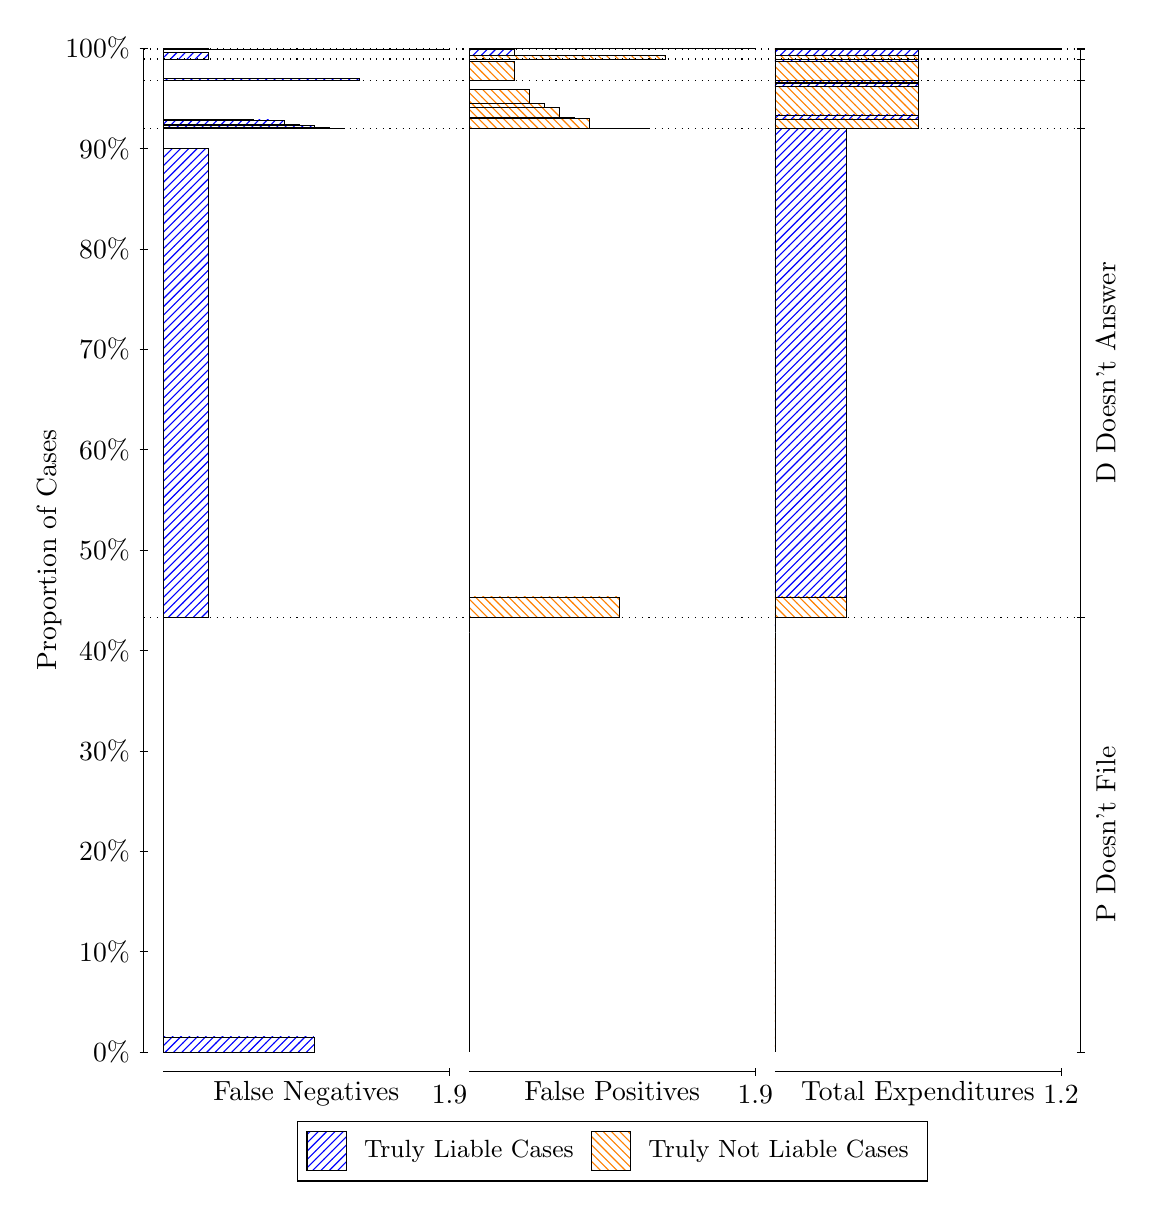
\begin{tikzpicture}
\draw[black, very thin] (1.5,1.75) -- (1.5,14.5);
\node[rotate=90, anchor=center] at (0.3, 8.125) {Proportion of Cases};
\draw[black, very thin] (1.45,1.75) -- (1.55,1.75);
\node[anchor=east] at (1.45, 1.75) {0\%};
\draw[black, very thin] (1.45,3.025) -- (1.55,3.025);
\node[anchor=east] at (1.45, 3.025) {10\%};
\draw[black, very thin] (1.45,4.3) -- (1.55,4.3);
\node[anchor=east] at (1.45, 4.3) {20\%};
\draw[black, very thin] (1.45,5.575) -- (1.55,5.575);
\node[anchor=east] at (1.45, 5.575) {30\%};
\draw[black, very thin] (1.45,6.85) -- (1.55,6.85);
\node[anchor=east] at (1.45, 6.85) {40\%};
\draw[black, very thin] (1.45,8.125) -- (1.55,8.125);
\node[anchor=east] at (1.45, 8.125) {50\%};
\draw[black, very thin] (1.45,9.4) -- (1.55,9.4);
\node[anchor=east] at (1.45, 9.4) {60\%};
\draw[black, very thin] (1.45,10.675) -- (1.55,10.675);
\node[anchor=east] at (1.45, 10.675) {70\%};
\draw[black, very thin] (1.45,11.95) -- (1.55,11.95);
\node[anchor=east] at (1.45, 11.95) {80\%};
\draw[black, very thin] (1.45,13.225) -- (1.55,13.225);
\node[anchor=east] at (1.45, 13.225) {90\%};
\draw[black, very thin] (1.45,14.5) -- (1.55,14.5);
\node[anchor=east] at (1.45, 14.5) {100\%};

\draw[black, very thin] (13.4,1.75) -- (13.4,14.5);
\draw[black, very thin] (13.35,1.75) -- (13.45,1.75);
\node[anchor=west] at (13.35, 1.75) {};
\draw[black, very thin] (13.35,7.2719) -- (13.45,7.2719);
\node[anchor=west] at (13.35, 7.2719) {};
\draw[black, very thin] (13.35,13.479) -- (13.45,13.479);
\node[anchor=west] at (13.35, 13.479) {};
\draw[black, very thin] (13.35,14.093) -- (13.45,14.093);
\node[anchor=west] at (13.35, 14.093) {};
\draw[black, very thin] (13.35,14.36) -- (13.45,14.36);
\node[anchor=west] at (13.35, 14.36) {};
\draw[black, very thin] (13.35,14.485) -- (13.45,14.485);
\node[anchor=west] at (13.35, 14.485) {};
\draw[black, very thin] (13.35,14.492) -- (13.45,14.492);
\node[anchor=west] at (13.35, 14.492) {};
\draw[black, very thin] (13.35,14.5) -- (13.45,14.5);
\node[anchor=west] at (13.35, 14.5) {};

\draw[black, very thin, pattern color=blue, pattern=north east lines] (1.75,1.75) rectangle (3.6623,1.9426);
\draw[black, very thin, pattern color=orange, pattern=north west lines] (1.75,1.9426) rectangle (1.75,7.2719);
\draw[black, very thin, pattern color=blue, pattern=north east lines] (1.75,7.2719) rectangle (2.3237,13.221);
\draw[black, very thin, pattern color=orange, pattern=north west lines] (1.75,13.221) rectangle (1.75,13.479);
\draw[black, very thin, pattern color=blue, pattern=north east lines] (1.75,13.479) rectangle (4.0447,13.484);
\draw[black, very thin, pattern color=blue, pattern=north east lines] (1.75,13.484) rectangle (3.8535,13.492);
\draw[black, very thin, pattern color=blue, pattern=north east lines] (1.75,13.492) rectangle (3.6623,13.517);
\draw[black, very thin, pattern color=blue, pattern=north east lines] (1.75,13.517) rectangle (3.4711,13.519);
\draw[black, very thin, pattern color=blue, pattern=north east lines] (1.75,13.519) rectangle (3.4711,13.533);
\draw[black, very thin, pattern color=blue, pattern=north east lines] (1.75,13.533) rectangle (3.2798,13.579);
\draw[black, very thin, pattern color=blue, pattern=north east lines] (1.75,13.579) rectangle (3.0886,13.588);
\draw[black, very thin, pattern color=blue, pattern=north east lines] (1.75,13.588) rectangle (2.8974,13.593);
\draw[black, very thin, pattern color=blue, pattern=north east lines] (1.75,13.593) rectangle (2.7061,13.594);
\draw[black, very thin, pattern color=blue, pattern=north east lines] (1.75,13.594) rectangle (2.5149,13.596);
\draw[black, very thin, pattern color=orange, pattern=north west lines] (1.75,13.596) rectangle (1.75,14.093);
\draw[black, very thin, pattern color=blue, pattern=north east lines] (1.75,14.093) rectangle (4.236,14.119);
\draw[black, very thin, pattern color=orange, pattern=north west lines] (1.75,14.119) rectangle (1.75,14.36);
\draw[black, very thin, pattern color=blue, pattern=north east lines] (1.75,14.36) rectangle (2.3237,14.443);
\draw[black, very thin, pattern color=orange, pattern=north west lines] (1.75,14.443) rectangle (1.75,14.485);
\draw[black, very thin, pattern color=blue, pattern=north east lines] (1.75,14.485) rectangle (5.3833,14.486);
\draw[black, very thin, pattern color=orange, pattern=north west lines] (1.75,14.486) rectangle (1.75,14.492);
\draw[black, very thin, pattern color=blue, pattern=north east lines] (1.75,14.492) rectangle (2.3237,14.499);
\draw[black, very thin, pattern color=orange, pattern=north west lines] (1.75,14.499) rectangle (1.75,14.5);
\draw[black, very thin, pattern color=orange, pattern=north west lines] (5.6333,1.75) rectangle (5.6333,7.0793);
\draw[black, very thin, pattern color=blue, pattern=north east lines] (5.6333,7.0793) rectangle (5.6333,7.2719);
\draw[black, very thin, pattern color=orange, pattern=north west lines] (5.6333,7.2719) rectangle (7.5456,7.5307);
\draw[black, very thin, pattern color=blue, pattern=north east lines] (5.6333,7.5307) rectangle (5.6333,13.479);
\draw[black, very thin, pattern color=orange, pattern=north west lines] (5.6333,13.479) rectangle (7.9281,13.479);
\draw[black, very thin, pattern color=orange, pattern=north west lines] (5.6333,13.479) rectangle (7.7368,13.479);
\draw[black, very thin, pattern color=orange, pattern=north west lines] (5.6333,13.479) rectangle (7.5456,13.481);
\draw[black, very thin, pattern color=orange, pattern=north west lines] (5.6333,13.481) rectangle (7.3544,13.483);
\draw[black, very thin, pattern color=orange, pattern=north west lines] (5.6333,13.483) rectangle (7.1632,13.602);
\draw[black, very thin, pattern color=orange, pattern=north west lines] (5.6333,13.602) rectangle (6.9719,13.623);
\draw[black, very thin, pattern color=orange, pattern=north west lines] (5.6333,13.623) rectangle (6.7807,13.748);
\draw[black, very thin, pattern color=orange, pattern=north west lines] (5.6333,13.748) rectangle (6.5895,13.797);
\draw[black, very thin, pattern color=orange, pattern=north west lines] (5.6333,13.797) rectangle (6.3982,13.976);
\draw[black, very thin, pattern color=blue, pattern=north east lines] (5.6333,13.976) rectangle (6.0158,13.979);
\draw[black, very thin, pattern color=blue, pattern=north east lines] (5.6333,13.979) rectangle (5.8246,13.979);
\draw[black, very thin, pattern color=blue, pattern=north east lines] (5.6333,13.979) rectangle (5.6333,14.093);
\draw[black, very thin, pattern color=orange, pattern=north west lines] (5.6333,14.093) rectangle (6.207,14.335);
\draw[black, very thin, pattern color=blue, pattern=north east lines] (5.6333,14.335) rectangle (5.6333,14.36);
\draw[black, very thin, pattern color=orange, pattern=north west lines] (5.6333,14.36) rectangle (8.1193,14.402);
\draw[black, very thin, pattern color=blue, pattern=north east lines] (5.6333,14.402) rectangle (6.207,14.485);
\draw[black, very thin, pattern color=orange, pattern=north west lines] (5.6333,14.485) rectangle (6.207,14.49);
\draw[black, very thin, pattern color=blue, pattern=north east lines] (5.6333,14.49) rectangle (5.6333,14.492);
\draw[black, very thin, pattern color=orange, pattern=north west lines] (5.6333,14.492) rectangle (9.2667,14.493);
\draw[black, very thin, pattern color=blue, pattern=north east lines] (5.6333,14.493) rectangle (7.3544,14.5);
\draw[black, very thin, pattern color=orange, pattern=north west lines] (9.5167,1.75) rectangle (9.5167,7.0793);
\draw[black, very thin, pattern color=blue, pattern=north east lines] (9.5167,7.0793) rectangle (9.5167,7.2719);
\draw[black, very thin, pattern color=orange, pattern=north west lines] (9.5167,7.2719) rectangle (10.425,7.5307);
\draw[black, very thin, pattern color=blue, pattern=north east lines] (9.5167,7.5307) rectangle (10.425,13.479);
\draw[black, very thin, pattern color=orange, pattern=north west lines] (9.5167,13.479) rectangle (11.333,13.599);
\draw[black, very thin, pattern color=blue, pattern=north east lines] (9.5167,13.599) rectangle (11.333,13.652);
\draw[black, very thin, pattern color=orange, pattern=north west lines] (9.5167,13.652) rectangle (11.333,14.008);
\draw[black, very thin, pattern color=blue, pattern=north east lines] (9.5167,14.008) rectangle (11.333,14.048);
\draw[black, very thin, pattern color=orange, pattern=north west lines] (9.5167,14.048) rectangle (11.333,14.069);
\draw[black, very thin, pattern color=blue, pattern=north east lines] (9.5167,14.069) rectangle (11.333,14.093);
\draw[black, very thin, pattern color=orange, pattern=north west lines] (9.5167,14.093) rectangle (11.333,14.335);
\draw[black, very thin, pattern color=blue, pattern=north east lines] (9.5167,14.335) rectangle (11.333,14.36);
\draw[black, very thin, pattern color=orange, pattern=north west lines] (9.5167,14.36) rectangle (11.333,14.402);
\draw[black, very thin, pattern color=blue, pattern=north east lines] (9.5167,14.402) rectangle (11.333,14.485);
\draw[black, very thin, pattern color=orange, pattern=north west lines] (9.5167,14.485) rectangle (13.15,14.49);
\draw[black, very thin, pattern color=blue, pattern=north east lines] (9.5167,14.49) rectangle (13.15,14.492);
\draw[black, very thin, pattern color=orange, pattern=north west lines] (9.5167,14.492) rectangle (13.15,14.493);
\draw[black, very thin, pattern color=blue, pattern=north east lines] (9.5167,14.493) rectangle (13.15,14.5);
\draw[black, dotted] (1.5,7.2719) -- (13.4,7.2719);
\draw[black, dotted] (1.5,13.479) -- (13.4,13.479);
\draw[black, dotted] (1.5,14.093) -- (13.4,14.093);
\draw[black, dotted] (1.5,14.36) -- (13.4,14.36);
\draw[black, dotted] (1.5,14.485) -- (13.4,14.485);
\draw[black, dotted] (1.5,14.492) -- (13.4,14.492);
\draw[black, very thin] (1.75,1.5) -- (5.3833,1.5);
\node[anchor=north] at (3.5667, 1.5) {False Negatives};
\draw[black, very thin] (5.3833,1.45) -- (5.3833,1.55);
\node[anchor=north] at (5.3833, 1.45) {1.9};

\draw[black, very thin] (5.6333,1.5) -- (9.2667,1.5);
\node[anchor=north] at (7.45, 1.5) {False Positives};
\draw[black, very thin] (9.2667,1.45) -- (9.2667,1.55);
\node[anchor=north] at (9.2667, 1.45) {1.9};

\draw[black, very thin] (9.5167,1.5) -- (13.15,1.5);
\node[anchor=north] at (11.333, 1.5) {Total Expenditures};
\draw[black, very thin] (13.15,1.45) -- (13.15,1.55);
\node[anchor=north] at (13.15, 1.45) {1.2};

\node[black, centered, rotate=90] at (13.72, 4.5109) {P Doesn't File};
\node[black, centered, rotate=90] at (13.72, 10.376) {D Doesn't Answer};






\draw (7.449999999999999,1.5) node[draw=none] (baseCoordinate) {};
\begin{scope}[align=center]
        \matrix[scale=0.5, draw=black, below=0.5cm of baseCoordinate, nodes={draw}, column sep=0.1cm]{
            \node[rectangle, draw, minimum width=0.5cm, minimum height=0.5cm, pattern=north east lines, pattern color=blue] {}; &
            \node[draw=none, font=\small] (B) {Truly Liable Cases}; &
            \node[rectangle, draw, minimum width=0.5cm, minimum height=0.5cm, pattern=north west lines, pattern color=orange] {}; &
            \node[draw=none, font=\small] (B) {Truly Not Liable Cases}; \\
            };
\end{scope}

\end{tikzpicture}
\end{document}